\documentclass[12pt,a4paper,two column]{article}
\usepackage[utf8]{inputenc}
\usepackage{mathtools}
\usepackage[a4paper, total={6in, 8in}, margin = 1in]{geometry}
\usepackage{enumitem}
\usepackage{graphicx}
\graphicspath{{images/}}
\usepackage{amsmath}

\title{ASSIGNMENT 2}
\author{Abhishek Kumar \\AI21BTECH11003}
\date{April 2022}
\begin{document}
	\maketitle
	\section*{Question 1(i)}
	\begin{align}
		f:R\xrightarrow{} R,f(x)= x^2\hspace{27}\\
		g:R\xrightarrow{} R,g(x)=2x^2+1
	\end{align}
	R is the set of Real Numbers.Find fog(x) and gof(x).
	\section*{Solution}
	Lets find  fog(x)
	\begin{align}
		f(x)=x^3,g(x)=2x^2+1 \nonumber\hspace{30}\\
		\implies f(g(x))= (2x^2+1)^3\nonumber\hspace{50}\\
		\implies fog(x)=8x^6+12x^4+6x^2+1
	\end{align}\\\\
	Lets find  gof(x)
	\begin{align}
		f(x)=x^3,g(x)=2x^2+1 \nonumber\hspace{30}\\
		\implies g(f(x))= 2(x^3)^2+1\nonumber\hspace{50}\\
		\implies fog(x)= 2x^6+1 \hspace{65}
	\end{align}
	\begin{figure}[h]
		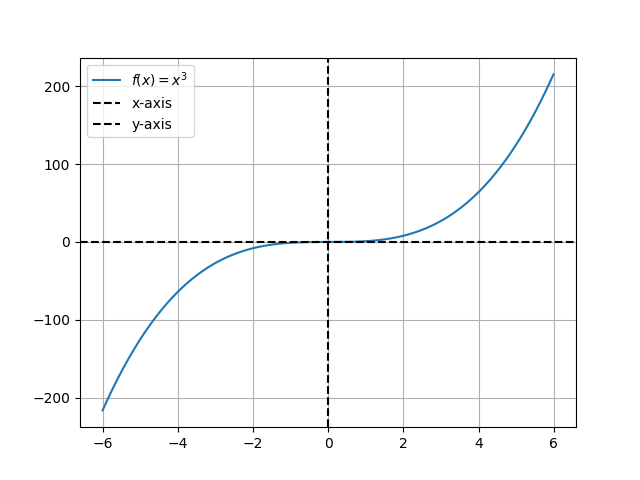
\includegraphics[width = \columnwidth]{f(x)}
		\caption{f(x)=$x^3$}
	\end{figure}
	\begin{figure}
		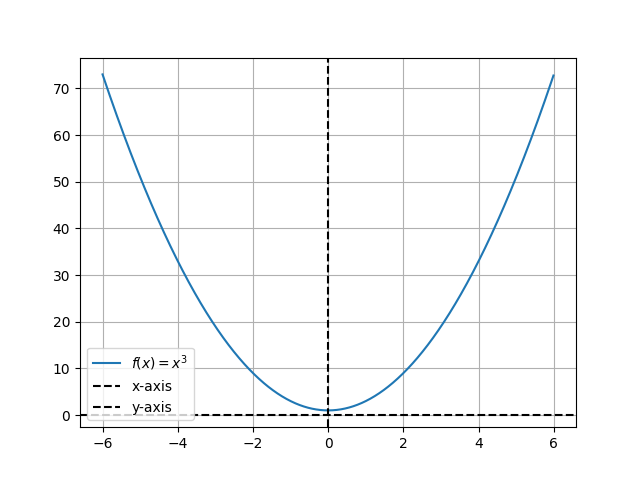
\includegraphics[width=\columnwidth]{g(x).png}
		\caption{g(x)=$2x^2+1$}
	\end{figure}
	\begin{figure}
		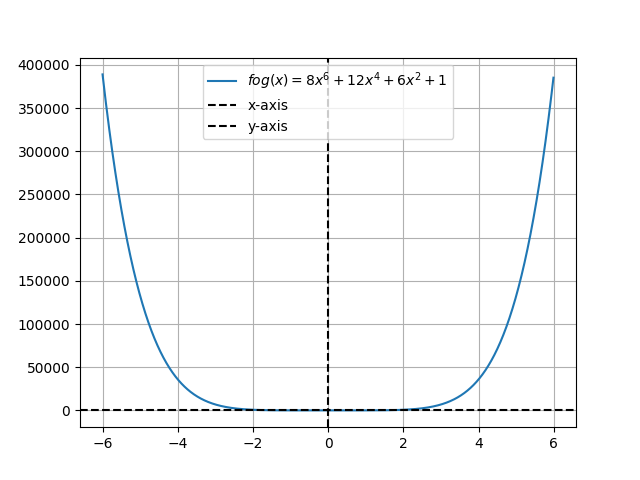
\includegraphics[width=\columnwidth]{fog(x).png}
		\caption{fog(x)=$8x^6+12x^4+6x^2+1$}
	\end{figure}
	\begin{figure}
		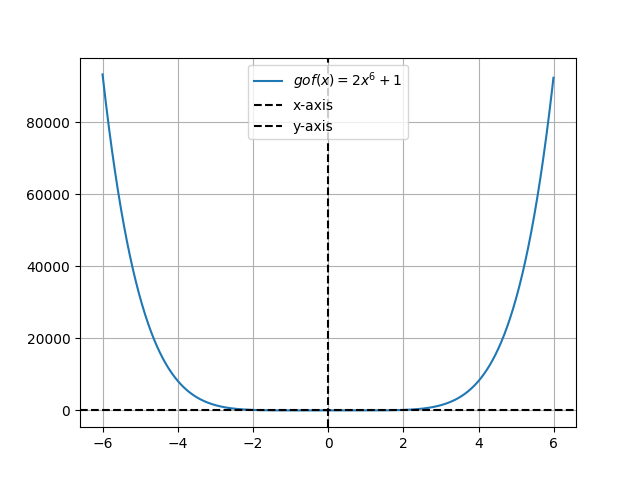
\includegraphics[width=\columnwidth]{gof(x).png}
		\caption{gof(x)=$2x^6+1$}
	\end{figure}
	
\end{document}
